\ffigbox[\FBwidth]{%
\caption{\centering Le pire des cas pour les zones de controle}\label{fig:dm1_ex02_f1}
}{
    \fbox{
        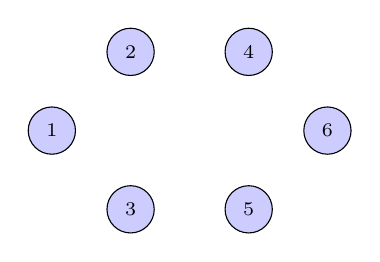
\begin{tikzpicture}[scale=1, main node/.style={circle, draw, fill=blue!20, inner sep=1pt, font=\scriptsize, minimum size=6mm, text=black}]
            % les sommets initiaux
            \node[main node] (1) at (0,0) {\(1\)};
            \node[main node] (2) at (1,1) {\(2\)};
            \node[main node] (3) at (1,-1) {\(3\)};
            
            \node[main node] (4) at (2.5,1) {\(4\)};
            \node[main node] (5) at (2.5,-1) {\(5\)};
            \node[main node] (6) at (3.5,0) {\(6\)};

        \end{tikzpicture}
    }
}